% !TeX spellcheck = en_US
\section{Verification}
In this section the verification of the example application HDL modules is being discussed. During the development of the example application HDL modules, the functional blocks are simulated separately. The HDL blocks are simulated with Mentor Graphics Questasim using a scripting language called Tool Command Language (TCL)~\cite{tcl}.

\subsection{Randomness of the data generator}
The heart of the example application HDL modules is the data generator. This provides data to the Wupper core. The data generator is based on the Linear Feedback Shift Register (LFSR). There are other techniques for generating (pseudo) random data such as the Linear Congruential Generator and Multiple Recursive Generators. The problem of these methods are the need of a lot of multiplication computing power~\cite{randomgen}. This requires a lot of digital logic / DSP slices.

It is important that the output data is random. To check this pattern Questasim is used for simulation. The first signal in Figure~\ref{fig:simapp} shows the output signal of the LFSR module using the approach by R.W. Ward and T.C.A Molteno~\cite{lfsrtable}. Questasim can plot the data in the waveform viewer which gives a nice overview of the randomness. 

\begin{figure}[h]
	\centering
	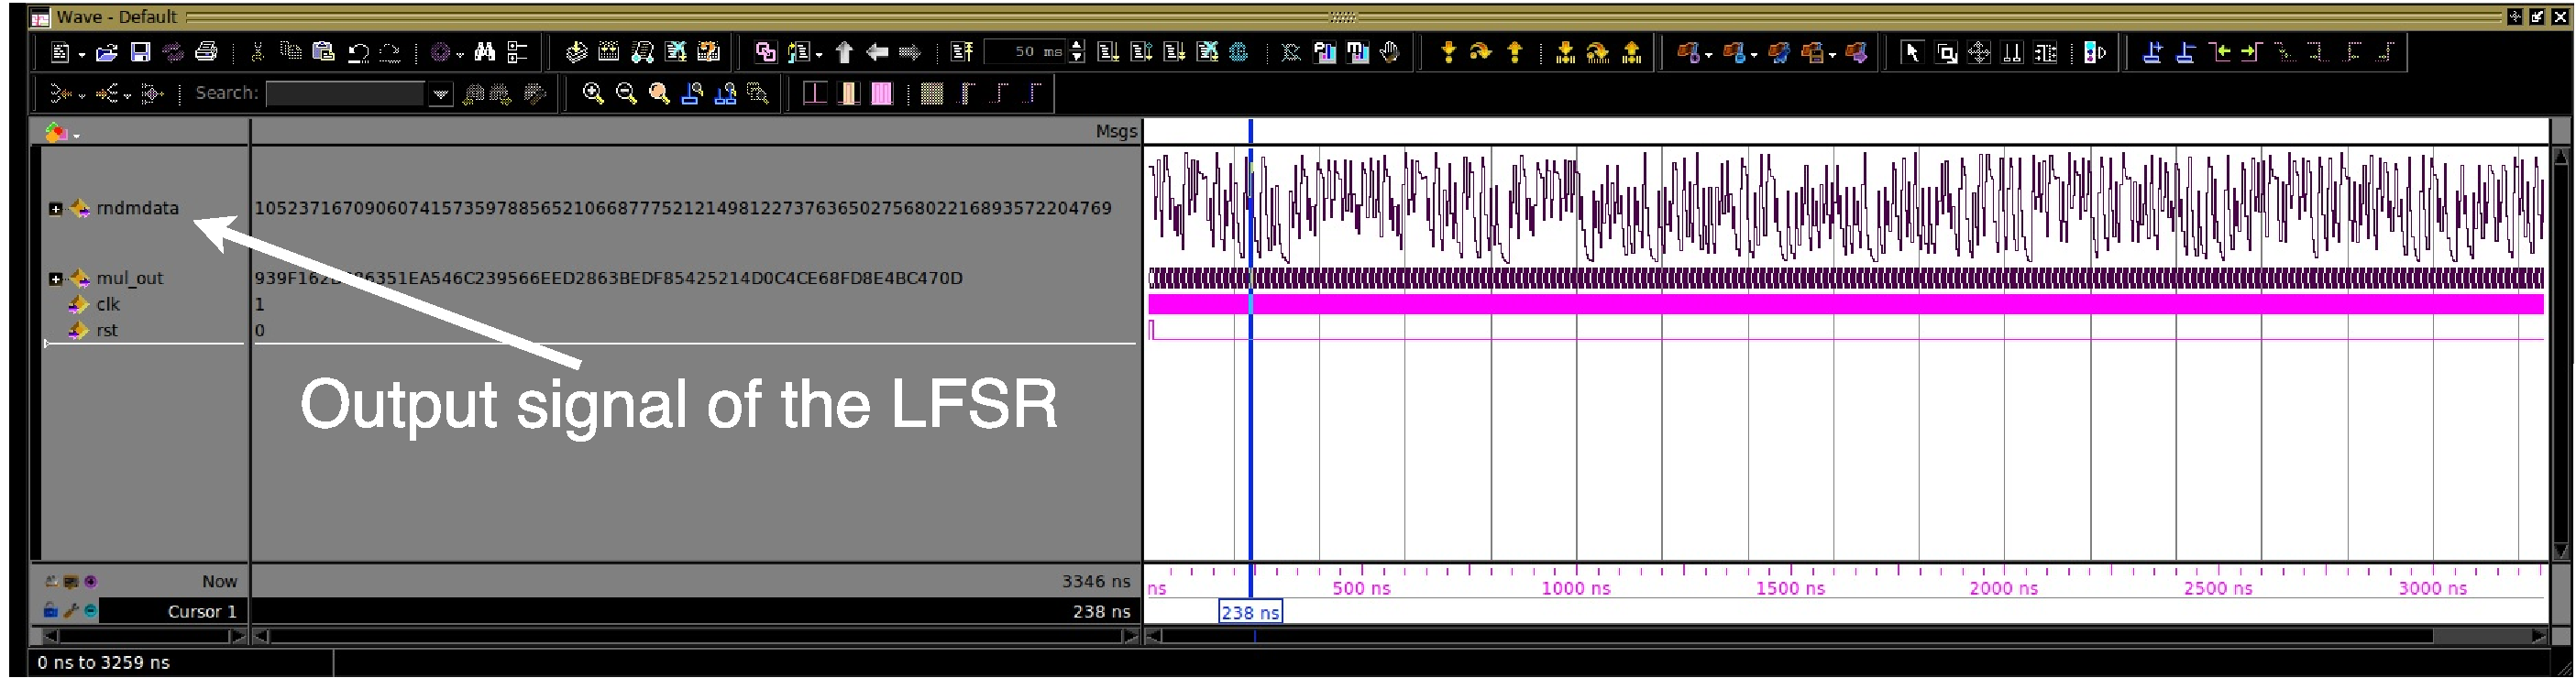
\includegraphics[width = 1 \textwidth]{figures/sim_lfsr_output.pdf}	
	\caption{Randomness of the data generator based on a 256-bits LFSR. }
	\label{fig:simapp}
\end{figure}


\subsection{Verification flow}
After an expected behaviour of the application HDL modules, the complete Wupper package needs to be verified. The expected behaviour of the full Wupper pacakage is that the output of the LFSR is first sent to a buffer in the PC memory. This buffer will later be transferred back into the FPGA by means of a DMA read cycle and fed into the input of the multipliers. Meanwhile, a second transfer is started simultaneously to transfer the multiplied data into a second buffer of PC memory.
Simulating the behaviour of transactions to PC memory is possible but very complex. In this case it is efficient to test the behavior real-time with Vivado's Integrated Logic Analyzer (ILA) ~\cite{ila}. ILA allows monitoring signals in real-time. The ILA core uses RAM blocks inside the FPGA as storage elements for the data in between acquisitions and subsequent transfers to host via the JTAG interface. It is therefore obvious that a combination of monitored signals and the depth of an acquisition will impact the resource consumption in the FPGA when equipped with debug probes. It is therefore crucial to carefully select the signals that one wants to monitor and the depth, i.e. number of samples, one wants to get per acquisition.

\newpage
When the probes are set properly and the triggers are armed, the next step in this process is operating the logic. This is done on the host PC via the Wupper-tools (described in Paragraph 3.3). The tools will activate the triggers and create an event. This event will acquire signal status which can be used for verifying the behaviour. This approach tests at the same time the HDL part and the low level software part. This approach and resources used during the verification is displayed below in Figure~\ref{fig:veriflow}.

\begin{figure}[h]
	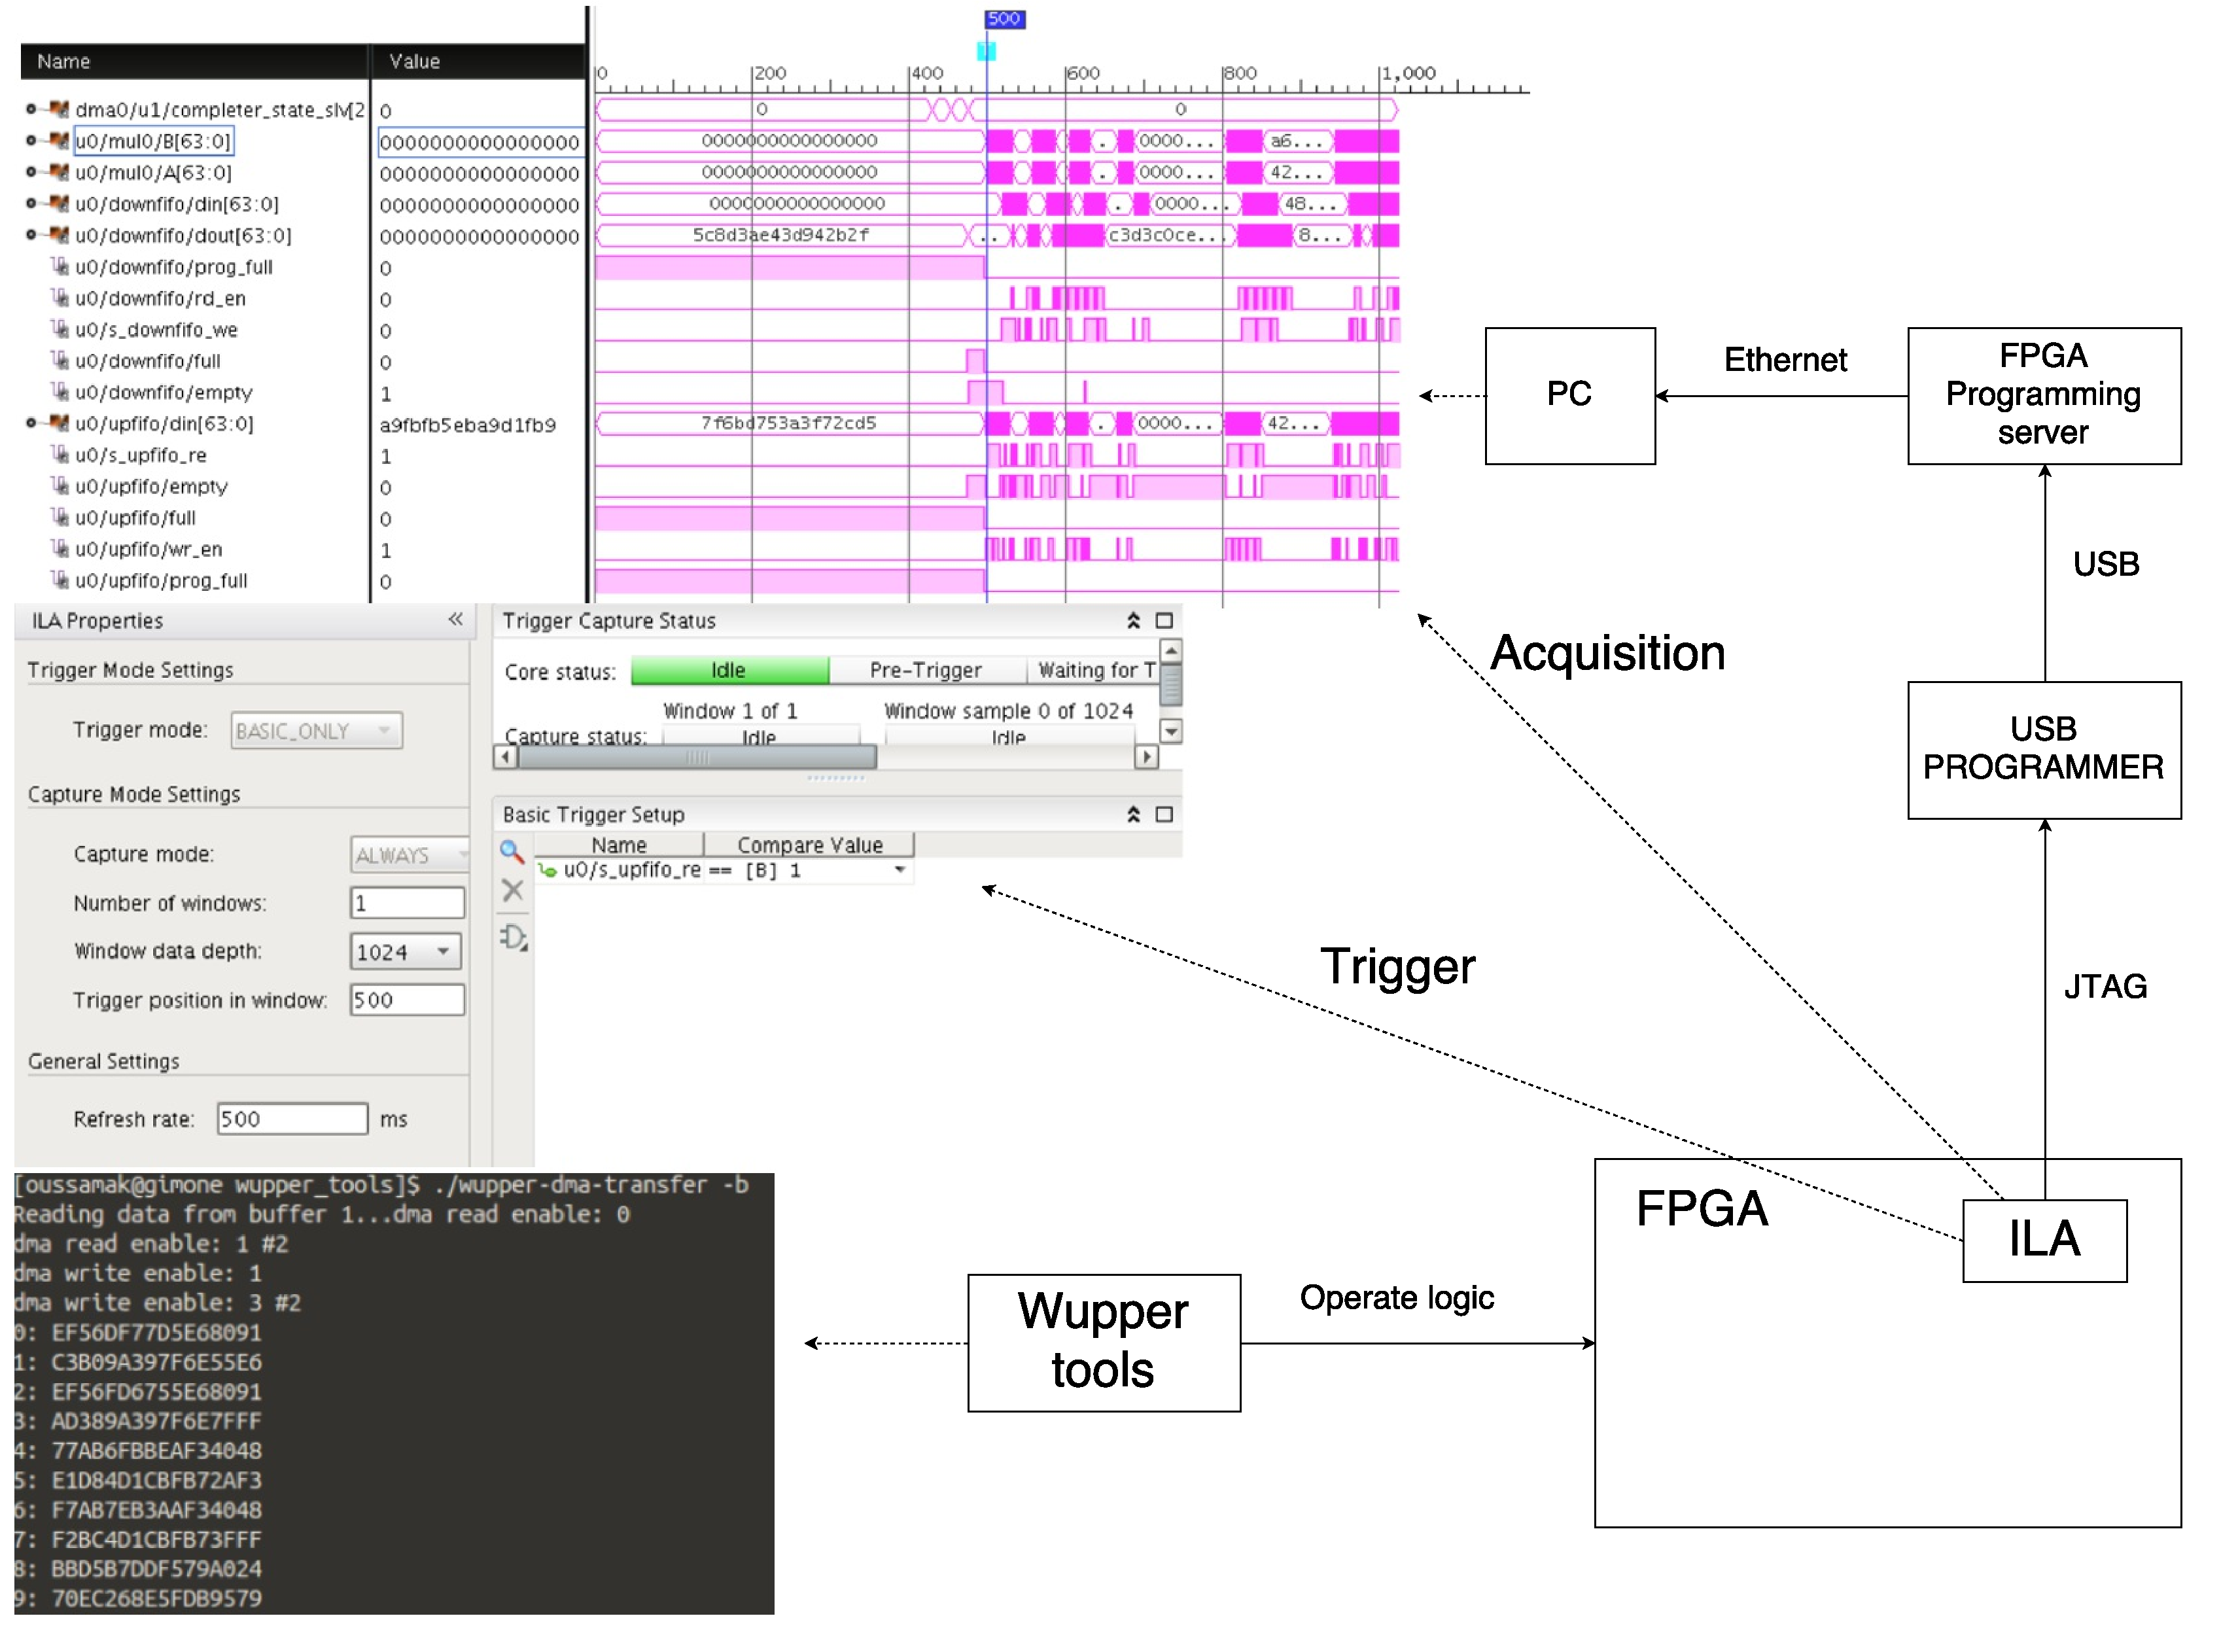
\includegraphics[width = 1 \textwidth]{figures/veriflow.pdf}	
	\caption{View of the verification flow}
	\label{fig:veriflow}
\end{figure}

The output of the LFSR is fed back to the input of the multipliers. To verify the multiplication, the tool Wupper-chaintest is developed. The tool activates the flow from the data generator to PC memory and back to the PC memory through the multipliers. As described in Section 3.3.2, the tool reserves two buffers inside the target PC. The data that is stored in buffer 2, are the inputs of the multipliers. This data is multiplied and verified with the output of the data that is stored in buffer 1. This is compared by the tool and returns an overview of errors that occur.

The high level software has the same purpose as the Wupper-tools. This makes it easy to implement it in the Wupper GUI. As mentioned before, the tools are based on programming languages C and C++ while Qt is based on C++. Which makes it possible to port the tools into Qt.

 
 
 
 \newpage